\documentclass[12pt]{article}
\usepackage{epsf}
\usepackage{amssymb}
\usepackage{enumitem}
\usepackage{amsmath}
\usepackage{tikz}
\usetikzlibrary{automata, positioning, arrows}

\title{aashlock-331-hw2}
\author{Aren Ashlock}
\date{February 2, 2024}

\setlength{\oddsidemargin}{-0.25in}
\setlength{\topmargin}{-0.5in}
\setlength{\headheight}{0cm}
\setlength{\headsep}{0cm}
\setlength{\textheight}{10in}
\setlength{\textwidth}{7in}
\setlength{\topskip}{0cm}

\begin{document}

\noindent\textbf{ComS 331 \quad Spring 2024 \quad Name: Aren Ashlock}

\begin{enumerate}

%----------------------------------- Q1 DONE -----------------------------------

\item Draw a DFA, simplified to the best of your abilities, that recognizes the language of \textbf{all} strings of $a$'s, $b$'s, and $c$'s where $a$ is never immediately followed by $b$.

\begin{tikzpicture}
    [node distance = 2cm]
    \node[state, initial, initial text=, accepting] (s1) {1};
    \node[state, accepting, right of=s1] (s2) {2};
    \node[state, right of=s2] (s3) {3};

    \path[->] (s1) edge [loop above] node {$b,c$} (s1);
    \path[->] (s1) edge [midway, above, bend left=10] node {$a$} (s2);
    \path[->] (s2) edge [midway, below, bend left=10] node {$c$} (s1);
    \path[->] (s2) edge [loop above] node {$a$} (s2);
    \path[->] (s2) edge [midway, above] node {$b$} (s3);
    \path[->] (s3) edge [loop right] node {$a,b,c$} (s3);
\end{tikzpicture}

%-------------------------------------------------------------------------------

%----------------------------------- Q2 DONE -----------------------------------

\item Draw a DFA, simplified to the best of your abilities, that recognizes the language\\ $L = \{w \in \{a, b\}^* : |w|_a \text{ mod } 3 = 0\}$.

\begin{tikzpicture}
    [node distance = 2cm]
    \node[state, initial, initial text=, accepting] (s1) {1};
    \node[state, right of=s1] (s2) {2};
    \node[state, right of=s2] (s3) {3};

    \path[->] (s1) edge [loop above] node {$b$} (s1);
    \path[->] (s1) edge [midway, above] node {$a$} (s2);
    \path[->] (s2) edge [loop above] node {$b$} (s2);
    \path[->] (s2) edge [midway, above] node {$a$} (s3);
    \path[->] (s3) edge [loop above] node {$b$} (s3);
    \path[->] (s3) edge [below, bend left=30] node {$a$} (s1);
\end{tikzpicture}

%-------------------------------------------------------------------------------

%----------------------------------- Q3 DONE -----------------------------------

\item Draw a DFA, simplified to the best of your abilities, that recognizes the language\\ $L = \{w \in \{a, b\}^* : w \text{ does not contain the substring } abba\}$.

\begin{tikzpicture}
    [node distance = 2cm]
    \node[state, initial, initial text=, accepting] (s1) {1};
    \node[state, accepting, right of=s1] (s2) {2};
    \node[state, accepting, right of=s2] (s3) {3};
    \node[state, accepting, right of=s3] (s4) {4};
    \node[state, right of=s4] (s5) {5};

    \path[->] (s1) edge [loop above] node {$b$} (s1);
    \path[->] (s1) edge [above] node {$a$} (s2);
    \path[->] (s2) edge [loop above] node {$a$} (s2);
    \path[->] (s2) edge [above, bend left=10] node {$b$} (s3);
    \path[->] (s3) edge [below, bend left=10] node {$a$} (s2);
    \path[->] (s3) edge [above] node {$b$} (s4);
    \path[->] (s4) edge [below, bend left=25] node {$b$} (s1);
    \path[->] (s4) edge [above] node {$a$} (s5);
    \path[->] (s5) edge [loop right] node {$a,b$} (s5);
\end{tikzpicture}

%-------------------------------------------------------------------------------

%----------------------------------- Q4 DONE -----------------------------------

\item Draw a DFA, simplified to the best of your abilities, that recognizes the language\\ $L = \{a^ib^j : (i + j) \text{ mod } 3 = 0\}$. Please explicitly draw the trap state, if needed, in your DFA.

\begin{tikzpicture}
    [node distance = 2cm]
    \node[state, initial, initial text=, accepting] (s1) {1};
    \node[state, right of=s1] (s2) {2};
    \node[state, right of=s2] (s3) {3};
    \node[state, below of=s1] (s4) {4};
    \node[state, right of=s4] (s5) {5};
    \node[state, accepting, right of=s5] (s6) {6};
    \node[state, below of=s5] (s7) {7};

    \path[->] (s1) edge [above] node {$a$} (s2);
    \path[->] (s1) edge [left] node {$b$} (s4);
    \path[->] (s2) edge [above] node {$a$} (s3);
    \path[->] (s2) edge [left] node {$b$} (s5);
    \path[->] (s3) edge [above, bend right=30] node {$a$} (s1);
    \path[->] (s3) edge [left] node {$b$} (s6);
    \path[->] (s4) edge [above] node {$b$} (s5);
    \path[->] (s4) edge [below] node {$a$} (s7);
    \path[->] (s5) edge [above] node {$b$} (s6);
    \path[->] (s5) edge [left] node {$a$} (s7);
    \path[->] (s6) edge [color=red, above, near start, bend left=30] node {$b$} (s4);
    \path[->] (s6) edge [left] node {$a$} (s7);
    \path[->] (s7) edge [loop below] node {$a,b$} (s7);
\end{tikzpicture}

\textbf{NOTE:} The red doesn't mean anything for this question. I just changed the color to establish what line the letter $b$ goes with.

%-------------------------------------------------------------------------------

\end{enumerate}
\end{document}